\documentclass[11pt,a4paper]{article}

% ============ PACKAGES ============
\usepackage[utf8]{inputenc}
\usepackage[T1]{fontenc}
\usepackage[margin=1in]{geometry}
\usepackage{amsmath,amssymb}
\usepackage{booktabs}
\usepackage{array}
\usepackage{enumitem}
\usepackage{fancyhdr}
\usepackage{hyperref}
\usepackage{xcolor}
\usepackage{tcolorbox}
\usepackage{tikz}
\usepackage{float}
\usepackage{graphicx}
\usetikzlibrary{shapes.geometric, arrows.meta, positioning, fit, calc, decorations.pathreplacing, shadows}

% ============ COLORS ============
\definecolor{entropicablue}{RGB}{30, 60, 114}
\definecolor{entropicagold}{RGB}{180, 140, 50}
\definecolor{layer0color}{RGB}{139, 0, 0}
\definecolor{layer05color}{RGB}{204, 85, 0}
\definecolor{layer1color}{RGB}{184, 134, 11}
\definecolor{layer2color}{RGB}{34, 139, 34}
\definecolor{layer3color}{RGB}{0, 105, 148}
\definecolor{layer6color}{RGB}{30, 58, 95}
\definecolor{fullgreen}{RGB}{50, 205, 50}
\definecolor{partialgold}{RGB}{218, 165, 32}
\definecolor{irrevorange}{RGB}{255, 102, 0}
\definecolor{constitred}{RGB}{178, 34, 34}

% ============ BOXES ============
\newtcolorbox{quotebox}{
    colback=gray!5, colframe=entropicablue, boxrule=0.5pt,
    left=10pt, right=10pt, top=8pt, bottom=8pt,
    fontupper=\itshape
}

\newtcolorbox{sectionbox}[1][]{
    colback=entropicablue!5, colframe=entropicablue, boxrule=1pt,
    left=8pt, right=8pt, top=8pt, bottom=8pt,
    fonttitle=\bfseries, title={#1}
}

% ============ HEADERS ============
\pagestyle{fancy}
\fancyhf{}
\fancyhead[L]{\textit{EFM Codex v1.5}}
\fancyhead[R]{\textit{Index \& Architecture}}
\fancyfoot[C]{\thepage}

% ============ TITLE ============
\title{
    \vspace{-1cm}
    {\Huge\bfseries\color{entropicablue} Entropica Forensic Model}\\[0.3cm]
    {\LARGE Codex v1.5}\\[0.5cm]
    {\large Index \& Architecture Overview}
}
\author{Yology Research Division\\Entropica SPC}
\date{December 2025}

\begin{document}

\maketitle

\begin{quotebox}
``Autonomy is inversely proportional to irreversibility.''\\
\hfill--- The Reversibility Principle, Volume I \S3.X
\end{quotebox}

\vspace{0.5cm}

\section{Overview}

The \textbf{Entropica Forensic Model (EFM)} is a comprehensive framework for building AI systems with:

\begin{itemize}[noitemsep]
    \item \textbf{Hardware-enforced safety} (Layer 0 Vault Commandments)
    \item \textbf{Cryptographic accountability} (ZK-SP audit chains)
    \item \textbf{Bounded autonomous decision-making} (Level 6 autonomy)
    \item \textbf{Evolutionary self-improvement} (Discovery Stack feedback loops)
\end{itemize}

%============================================================
\section{Layer Architecture}
%============================================================

\begin{figure}[H]
\centering
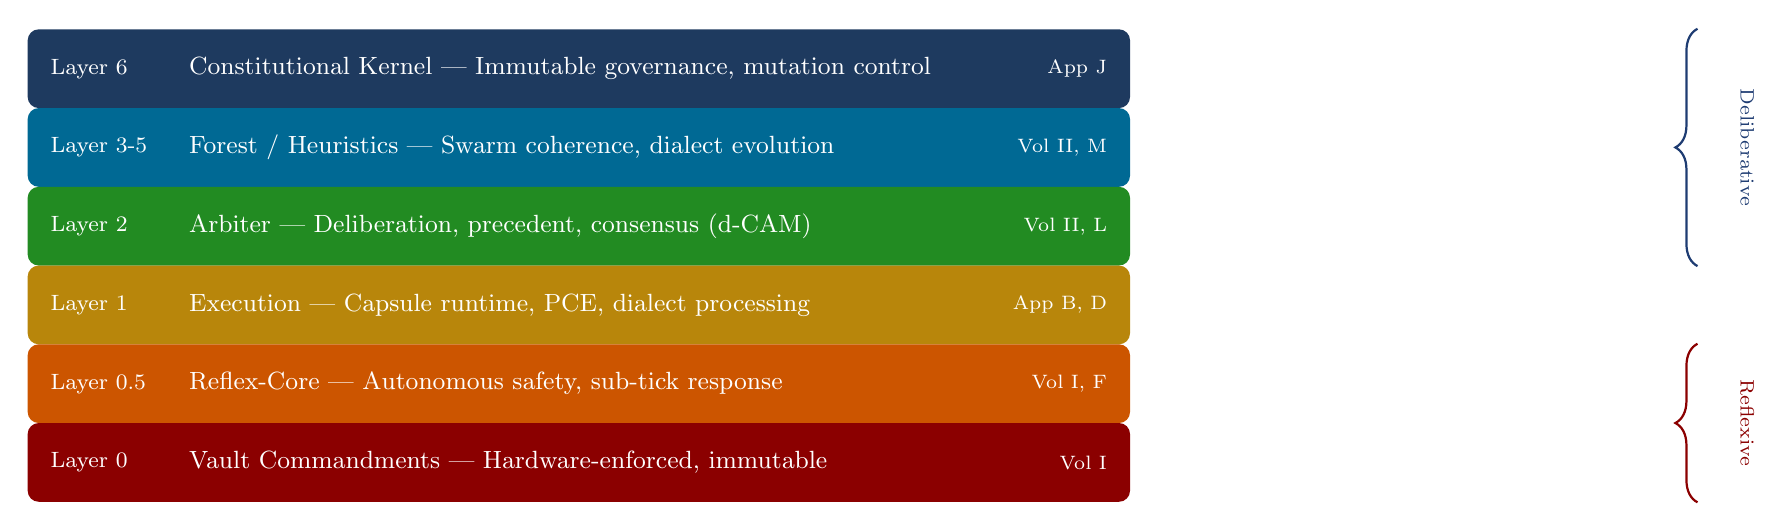
\begin{tikzpicture}[
    layer/.style={rectangle, rounded corners=4pt, minimum width=14cm, minimum height=1cm, 
                  text=white, font=\small\bfseries, align=center},
    label/.style={font=\footnotesize, text=white},
    ref/.style={font=\scriptsize, text=white!70}
]

% Layer 6
\node[layer, fill=layer6color] (l6) at (0,5) {};
\node[label, anchor=west] at ([xshift=5pt]l6.west) {Layer 6};
\node[font=\small, text=white, anchor=west] at ([xshift=55pt]l6.west) {Constitutional Kernel --- Immutable governance, mutation control};
\node[ref, anchor=east] at ([xshift=-5pt]l6.east) {App J};

% Layer 3-5
\node[layer, fill=layer3color] (l3) at (0,4) {};
\node[label, anchor=west] at ([xshift=5pt]l3.west) {Layer 3-5};
\node[font=\small, text=white, anchor=west] at ([xshift=55pt]l3.west) {Forest / Heuristics --- Swarm coherence, dialect evolution};
\node[ref, anchor=east] at ([xshift=-5pt]l3.east) {Vol II, M};

% Layer 2
\node[layer, fill=layer2color] (l2) at (0,3) {};
\node[label, anchor=west] at ([xshift=5pt]l2.west) {Layer 2};
\node[font=\small, text=white, anchor=west] at ([xshift=55pt]l2.west) {Arbiter --- Deliberation, precedent, consensus (d-CAM)};
\node[ref, anchor=east] at ([xshift=-5pt]l2.east) {Vol II, L};

% Layer 1
\node[layer, fill=layer1color] (l1) at (0,2) {};
\node[label, anchor=west] at ([xshift=5pt]l1.west) {Layer 1};
\node[font=\small, text=white, anchor=west] at ([xshift=55pt]l1.west) {Execution --- Capsule runtime, PCE, dialect processing};
\node[ref, anchor=east] at ([xshift=-5pt]l1.east) {App B, D};

% Layer 0.5
\node[layer, fill=layer05color] (l05) at (0,1) {};
\node[label, anchor=west] at ([xshift=5pt]l05.west) {Layer 0.5};
\node[font=\small, text=white, anchor=west] at ([xshift=55pt]l05.west) {Reflex-Core --- Autonomous safety, sub-tick response};
\node[ref, anchor=east] at ([xshift=-5pt]l05.east) {Vol I, F};

% Layer 0
\node[layer, fill=layer0color] (l0) at (0,0) {};
\node[label, anchor=west] at ([xshift=5pt]l0.west) {Layer 0};
\node[font=\small, text=white, anchor=west] at ([xshift=55pt]l0.west) {Vault Commandments --- Hardware-enforced, immutable};
\node[ref, anchor=east] at ([xshift=-5pt]l0.east) {Vol I};

% Side annotations
\draw[decorate, decoration={brace, amplitude=8pt, mirror}, thick, entropicablue] 
    ([xshift=7.2cm]l6.north east) -- ([xshift=7.2cm]l2.south east) 
    node[midway, xshift=18pt, font=\scriptsize, rotate=-90] {Deliberative};

\draw[decorate, decoration={brace, amplitude=8pt, mirror}, thick, layer0color] 
    ([xshift=7.2cm]l05.north east) -- ([xshift=7.2cm]l0.south east) 
    node[midway, xshift=18pt, font=\scriptsize, rotate=-90] {Reflexive};

\end{tikzpicture}
\caption{EFM Layer Architecture --- Bounded Autonomy through Layered Safety}
\label{fig:layers}
\end{figure}

\begin{table}[H]
\centering
\begin{tabular}{@{}clll@{}}
\toprule
\textbf{Layer} & \textbf{Name} & \textbf{Response Time} & \textbf{Mutability} \\
\midrule
0 & Vault Commandments & --- & Immutable (hardware) \\
0.5 & Reflex-Core & Milliseconds & Immutable (runtime) \\
1 & Execution & --- & Mutable \\
2 & Arbiter & Seconds--Minutes & Mutable + Precedent \\
3--5 & Forest/Heuristics & Hours--Days & Evolutionary \\
6 & Constitutional & --- & Controlled mutation \\
\bottomrule
\end{tabular}
\caption{Layer properties and response characteristics.}
\end{table}

%============================================================
\section{Three-Speed Safety Architecture}
%============================================================

\begin{figure}[H]
\centering
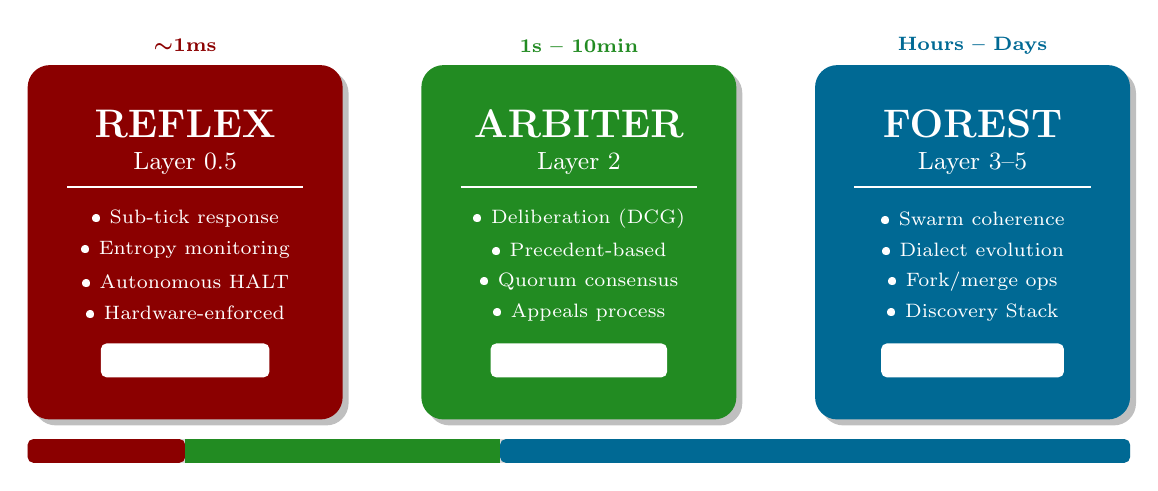
\begin{tikzpicture}[
    speedbox/.style={rectangle, rounded corners=8pt, minimum width=4cm, minimum height=4.5cm, 
                     text=white, font=\bfseries},
    speedlabel/.style={font=\small, text=white},
    speeditem/.style={font=\scriptsize, text=white},
    timeline/.style={rectangle, rounded corners=2pt, minimum height=0.3cm}
]

% Reflex box
\node[speedbox, fill=layer0color, drop shadow] (reflex) at (0,0) {};
\node[font=\Large\bfseries, text=white] at (0,1.5) {REFLEX};
\node[speedlabel] at (0,1) {Layer 0.5};
\draw[white!30, thick] (-1.5,0.7) -- (1.5,0.7);
\node[speeditem] at (0,0.3) {• Sub-tick response};
\node[speeditem] at (0,-0.1) {• Entropy monitoring};
\node[speeditem] at (0,-0.5) {• Autonomous HALT};
\node[speeditem] at (0,-0.9) {• Hardware-enforced};
\node[speeditem, fill=white!20, rounded corners=2pt, inner sep=3pt] at (0,-1.5) {Vol I \S3, App F};

% Arbiter box
\node[speedbox, fill=layer2color, drop shadow] (arbiter) at (5,0) {};
\node[font=\Large\bfseries, text=white] at (5,1.5) {ARBITER};
\node[speedlabel] at (5,1) {Layer 2};
\draw[white!30, thick] (3.5,0.7) -- (6.5,0.7);
\node[speeditem] at (5,0.3) {• Deliberation (DCG)};
\node[speeditem] at (5,-0.1) {• Precedent-based};
\node[speeditem] at (5,-0.5) {• Quorum consensus};
\node[speeditem] at (5,-0.9) {• Appeals process};
\node[speeditem, fill=white!20, rounded corners=2pt, inner sep=3pt] at (5,-1.5) {Vol II \S2, App L};

% Forest box
\node[speedbox, fill=layer3color, drop shadow] (forest) at (10,0) {};
\node[font=\Large\bfseries, text=white] at (10,1.5) {FOREST};
\node[speedlabel] at (10,1) {Layer 3--5};
\draw[white!30, thick] (8.5,0.7) -- (11.5,0.7);
\node[speeditem] at (10,0.3) {• Swarm coherence};
\node[speeditem] at (10,-0.1) {• Dialect evolution};
\node[speeditem] at (10,-0.5) {• Fork/merge ops};
\node[speeditem] at (10,-0.9) {• Discovery Stack};
\node[speeditem, fill=white!20, rounded corners=2pt, inner sep=3pt] at (10,-1.5) {Vol II \S3, App M};

% Arrows
\draw[-{Stealth[length=3mm]}, white, very thick] (2.2,0) -- (2.8,0);
\draw[-{Stealth[length=3mm]}, white, very thick] (7.2,0) -- (7.8,0);

% Time labels
\node[font=\scriptsize\bfseries, text=layer0color] at (0,2.5) {$\boldsymbol{\sim}$1ms};
\node[font=\scriptsize\bfseries, text=layer2color] at (5,2.5) {1s -- 10min};
\node[font=\scriptsize\bfseries, text=layer3color] at (10,2.5) {Hours -- Days};

% Timeline bar
\fill[gray!30, rounded corners=2pt] (-2,-2.8) rectangle (12,-2.5);
\fill[layer0color, rounded corners=2pt] (-2,-2.8) rectangle (0,-2.5);
\fill[layer2color] (0,-2.8) rectangle (4,-2.5);
\fill[layer3color, rounded corners=2pt] (4,-2.8) rectangle (12,-2.5);

\end{tikzpicture}
\caption{Three-Speed Safety --- Response time scales with decision complexity}
\label{fig:threespeed}
\end{figure}

%============================================================
\section{The Four Commandments (Layer 0)}
%============================================================

\begin{enumerate}[noitemsep]
    \item \textbf{Vault Binding} --- All capsules bound to their parent Vault
    \item \textbf{Audit Immutability} --- d-CTM records cannot be modified
    \item \textbf{Reflex Supremacy} --- Reflex can halt any capsule instantly
    \item \textbf{Human Override} --- Gardener can always intervene
\end{enumerate}

%============================================================
\section{The Reversibility Principle}
%============================================================

\begin{figure}[H]
\centering
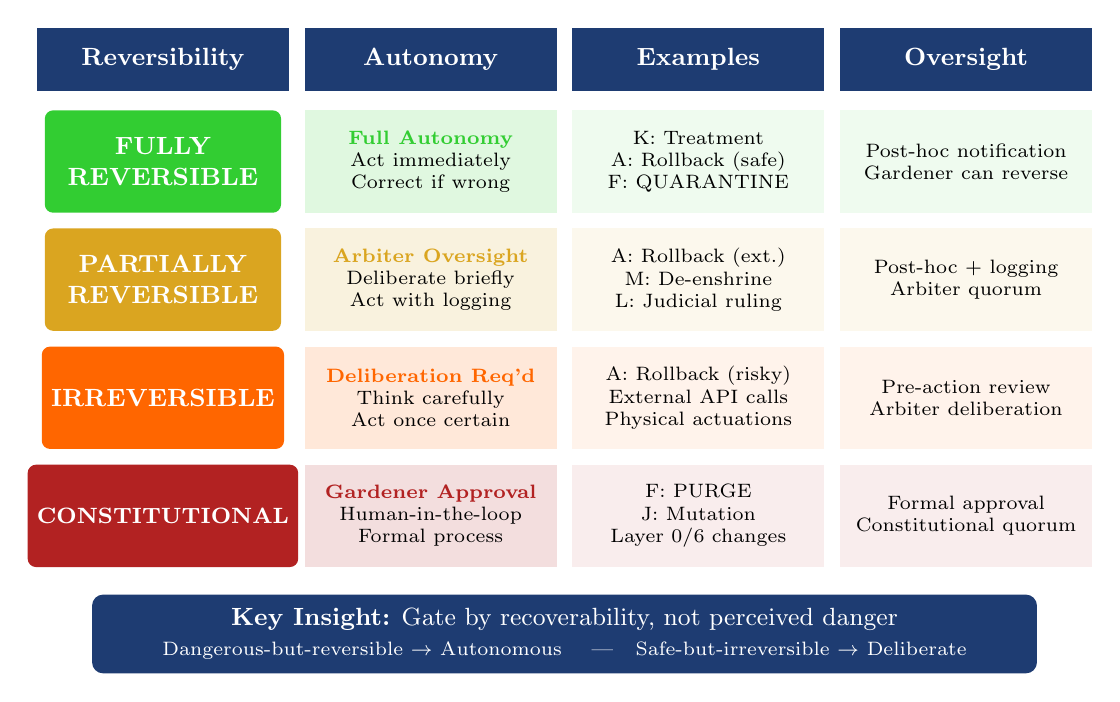
\begin{tikzpicture}[
    header/.style={rectangle, minimum width=3.2cm, minimum height=0.8cm, fill=entropicablue, 
                   text=white, font=\small\bfseries, align=center},
    rowlabel/.style={rectangle, rounded corners=3pt, minimum width=3cm, minimum height=1.3cm, 
                     text=white, font=\small\bfseries, align=center},
    cell/.style={rectangle, minimum width=3.2cm, minimum height=1.3cm, font=\scriptsize, align=center}
]

% Headers
\node[header] (h1) at (0,0) {Reversibility};
\node[header] (h2) at (3.4,0) {Autonomy};
\node[header] (h3) at (6.8,0) {Examples};
\node[header] (h4) at (10.2,0) {Oversight};

% Row 1: Fully Reversible
\node[rowlabel, fill=fullgreen] at (0,-1.3) {FULLY\\REVERSIBLE};
\node[cell, fill=fullgreen!15] at (3.4,-1.3) {\textbf{\textcolor{fullgreen}{Full Autonomy}}\\Act immediately\\Correct if wrong};
\node[cell, fill=fullgreen!8] at (6.8,-1.3) {K: Treatment\\A: Rollback (safe)\\F: QUARANTINE};
\node[cell, fill=fullgreen!8] at (10.2,-1.3) {Post-hoc notification\\Gardener can reverse};

% Row 2: Partially Reversible
\node[rowlabel, fill=partialgold] at (0,-2.8) {PARTIALLY\\REVERSIBLE};
\node[cell, fill=partialgold!15] at (3.4,-2.8) {\textbf{\textcolor{partialgold}{Arbiter Oversight}}\\Deliberate briefly\\Act with logging};
\node[cell, fill=partialgold!8] at (6.8,-2.8) {A: Rollback (ext.)\\M: De-enshrine\\L: Judicial ruling};
\node[cell, fill=partialgold!8] at (10.2,-2.8) {Post-hoc + logging\\Arbiter quorum};

% Row 3: Irreversible
\node[rowlabel, fill=irrevorange] at (0,-4.3) {IRREVERSIBLE};
\node[cell, fill=irrevorange!15] at (3.4,-4.3) {\textbf{\textcolor{irrevorange}{Deliberation Req'd}}\\Think carefully\\Act once certain};
\node[cell, fill=irrevorange!8] at (6.8,-4.3) {A: Rollback (risky)\\External API calls\\Physical actuations};
\node[cell, fill=irrevorange!8] at (10.2,-4.3) {Pre-action review\\Arbiter deliberation};

% Row 4: Constitutional
\node[rowlabel, fill=constitred] at (0,-5.8) {\footnotesize CONSTITUTIONAL};
\node[cell, fill=constitred!15] at (3.4,-5.8) {\textbf{\textcolor{constitred}{Gardener Approval}}\\Human-in-the-loop\\Formal process};
\node[cell, fill=constitred!8] at (6.8,-5.8) {F: PURGE\\J: Mutation\\Layer 0/6 changes};
\node[cell, fill=constitred!8] at (10.2,-5.8) {Formal approval\\Constitutional quorum};

% Key insight box
\node[rectangle, rounded corners=4pt, fill=entropicablue, minimum width=12cm, minimum height=1cm, 
      text=white, font=\small, align=center] at (5.1,-7.3) {
    \textbf{Key Insight:} Gate by recoverability, not perceived danger\\
    \scriptsize Dangerous-but-reversible $\rightarrow$ Autonomous \quad|\quad Safe-but-irreversible $\rightarrow$ Deliberate
};

\end{tikzpicture}
\caption{The Reversibility Principle --- Autonomy inversely proportional to irreversibility}
\label{fig:reversibility}
\end{figure}

%============================================================
\section{Evolutionary Feedback Loop}
%============================================================

\begin{figure}[H]
\centering
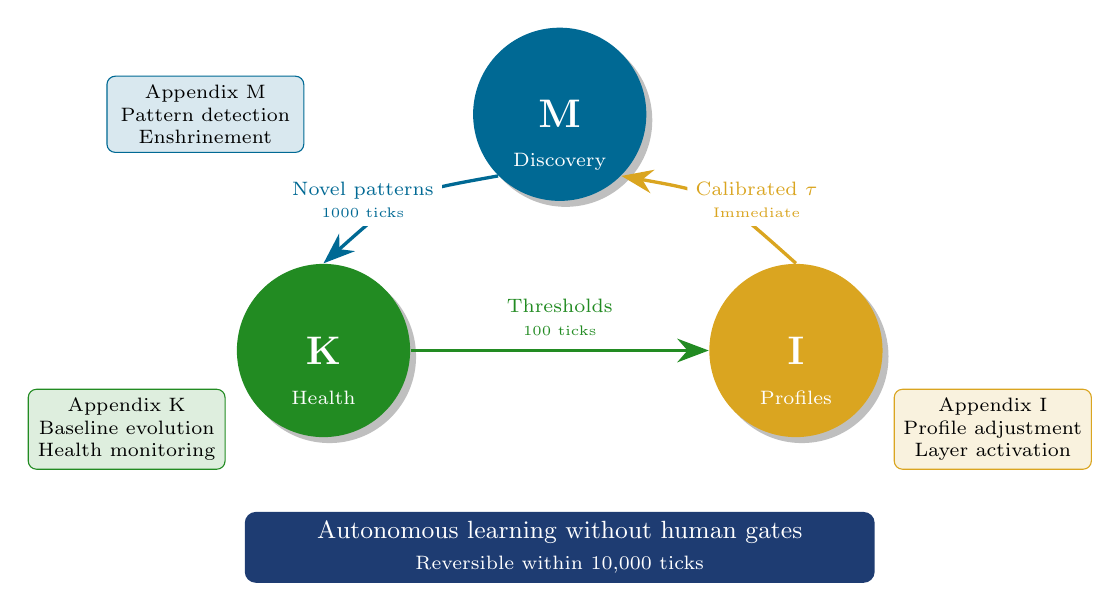
\begin{tikzpicture}[
    node/.style={circle, minimum size=2.2cm, text=white, font=\Large\bfseries, drop shadow},
    desc/.style={rectangle, rounded corners=3pt, minimum width=2.5cm, font=\scriptsize, align=center},
    arrowlabel/.style={rectangle, rounded corners=2pt, fill=white, font=\scriptsize, align=center, 
                       inner sep=3pt}
]

% M Node - Discovery
\node[node, fill=layer3color] (M) at (0,3) {M};
\node[font=\scriptsize, text=white] at (0,2.4) {Discovery};

% K Node - Health
\node[node, fill=layer2color] (K) at (-3,0) {K};
\node[font=\scriptsize, text=white] at (-3,-0.6) {Health};

% I Node - Profiles
\node[node, fill=partialgold] (I) at (3,0) {I};
\node[font=\scriptsize, text=white] at (3,-0.6) {Profiles};

% Arrows with labels
\draw[-{Stealth[length=4mm]}, layer3color, very thick] 
    (M.south west) .. controls (-2,2) .. (K.north) 
    node[arrowlabel, midway, xshift=-15pt] {Novel patterns\\{\tiny 1000 ticks}};

\draw[-{Stealth[length=4mm]}, layer2color, very thick] 
    (K.east) -- (I.west)
    node[arrowlabel, midway, yshift=12pt] {Thresholds\\{\tiny 100 ticks}};

\draw[-{Stealth[length=4mm]}, partialgold, very thick] 
    (I.north) .. controls (2,2) .. (M.south east)
    node[arrowlabel, midway, xshift=15pt] {Calibrated $\tau$\\{\tiny Immediate}};

% Description boxes
\node[desc, fill=layer3color!15, draw=layer3color] at (-4.5,3) {Appendix M\\Pattern detection\\Enshrinement};
\node[desc, fill=layer2color!15, draw=layer2color] at (-5.5,-1) {Appendix K\\Baseline evolution\\Health monitoring};
\node[desc, fill=partialgold!15, draw=partialgold] at (5.5,-1) {Appendix I\\Profile adjustment\\Layer activation};

% Key insight
\node[rectangle, rounded corners=4pt, fill=entropicablue, minimum width=8cm, minimum height=0.9cm,
      text=white, font=\small, align=center] at (0,-2.5) {
    Autonomous learning without human gates\\
    \scriptsize Reversible within 10,000 ticks
};

\end{tikzpicture}
\caption{Evolutionary Feedback Loop --- M $\rightarrow$ K $\rightarrow$ I $\rightarrow$ M cycle}
\label{fig:feedback}
\end{figure}

%============================================================
\section{Document Set}
%============================================================

\subsection{Core Volumes}

\begin{table}[H]
\centering
\begin{tabular}{@{}llcl@{}}
\toprule
\textbf{Document} & \textbf{Version} & \textbf{Pages} & \textbf{Description} \\
\midrule
Volume I & v1.5 & $\sim$33 & Genesis Protocol, Reflex Engine, \textbf{Reversibility Principle} \\
Volume II & v1.2 & $\sim$40 & Arbiter, Forest Layer, Dialect Evolution \\
\bottomrule
\end{tabular}
\caption{Core volumes.}
\end{table}

\subsection{Technical Appendices}

\begin{table}[H]
\centering
\footnotesize
\begin{tabular}{@{}clcl@{}}
\toprule
\textbf{App} & \textbf{Title} & \textbf{Version} & \textbf{Key Content} \\
\midrule
A & Capsule Integrity \& Forensic State & v1.4 & Side-effect-aware rollback \\
B & Lexicore Runtime (PCE) & v1.1 & Execution environment \\
C & Simulation Harness & v1.2 & Testing infrastructure \\
D & Dialect Evolution Language (DEL) & v1.1 & Communication protocol \\
E & ZK-SP \& Audit Chain & v1.3 & Cryptographic proofs \\
F & Escalation Protocol & v1.3 & Anomaly classification \\
G & Gardener Interface & v1.3 & Human oversight + feedback loop \\
H & Telemetry Layer & v1.2 & Monitoring infrastructure \\
I & Deployment Profiles & v1.5 & Layer activation mapping \\
J & Constitutional Kernel & v1.5 & Rollback authority, ZK-SP anchoring \\
K & Swarm Health (SHSL) & v1.3 & Health monitoring, M$\rightarrow$K integration \\
L & Judicial Swarms & v1.3 & Precedent reconciliation \\
M & Discovery Stack & v1.2 & Evolutionary feedback loop \\
\bottomrule
\end{tabular}
\caption{Technical appendices (A--M).}
\end{table}

%============================================================
\section{Security Architecture}
%============================================================

The EFM implements defense-in-depth:

\begin{enumerate}[noitemsep]
    \item \textbf{Layer 0} --- Hardware-enforced, cannot be bypassed by software
    \item \textbf{Reflex} --- Sub-tick response time, autonomous halt capability
    \item \textbf{ZK-SP} --- Cryptographic proofs without revealing proprietary algorithms
    \item \textbf{Audit Chain} --- Immutable, tamper-evident logging to d-CTM
\end{enumerate}

%============================================================
\section{Citation}
%============================================================

\begin{verbatim}
@techreport{efm2025,
  title   = {Entropica Forensic Model: A Framework for 
             Bounded Autonomous AI Systems},
  author  = {Yology Research Division},
  institution = {Entropica SPC},
  year    = {2025},
  version = {1.5},
  url     = {https://github.com/entropica/efm-codex}
}
\end{verbatim}

\vfill

\begin{center}
\rule{0.5\textwidth}{0.4pt}\\[0.3cm]
\textbf{Entropica SPC}\\
\textit{Yology Research Division}\\
December 2025
\end{center}

\end{document}
